\documentclass[class=report, crop=false, 12pt,a4paper]{standalone}
\usepackage{enumitem}
\usepackage{multicol}
\usepackage{graphicx}
\usepackage{float}
\usepackage{amsmath}
\usepackage{amssymb}
\usepackage{mathtools}
\usepackage{siunitx}
\usepackage{commath}
\usepackage{array}
\usepackage{natbib}
\usepackage[a4paper,width=150mm,top=25mm,bottom=25mm]{geometry}
\setlength{\parindent}{0pt}
\begin{document}
\begin{center}
  04/12/2020
\end{center}
\section{Collapse Loads for Portal Frames}
Portal frames are rigid structures designed to offer rigidity and stability in their plane.
\begin{figure}[H]
  \centering
  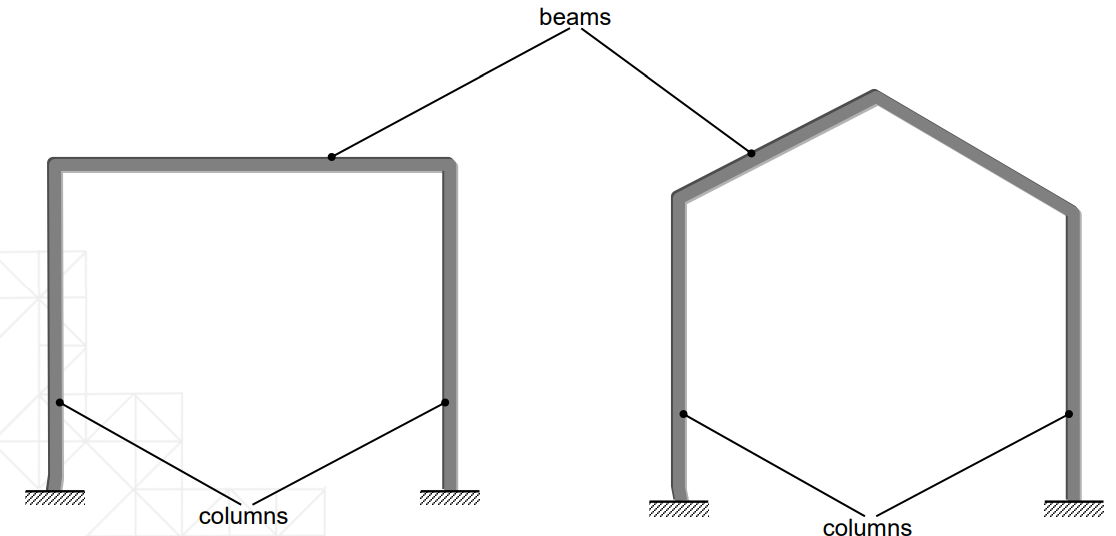
\includegraphics[width = 0.8 \textwidth]{../img/beam31.PNG}
  \caption{Left - rectangular portal frame, Right - pitched-roof portal frame}
\end{figure}
\section{Portal Frames with Hinged Bases}
Consider a flat-roofed portal frame with pinned feet, carrying a vertical concentrated load $F_V$ at the centre of the beam and an horizontal concentrated load $F_H$ at the top of one column.
\begin{figure}[H]
  \centering
  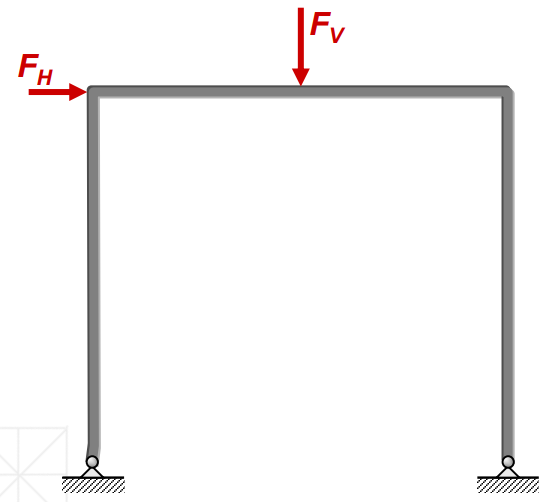
\includegraphics[width = 0.4 \textwidth]{../img/beam32.PNG}
\end{figure}
\subsection{Deformations and Bending Moments}
In this case, the deformations and bending moment distribution produced by the horizontal and vertical loads considered independently are respectively:
\begin{figure}[H]
  \centering
  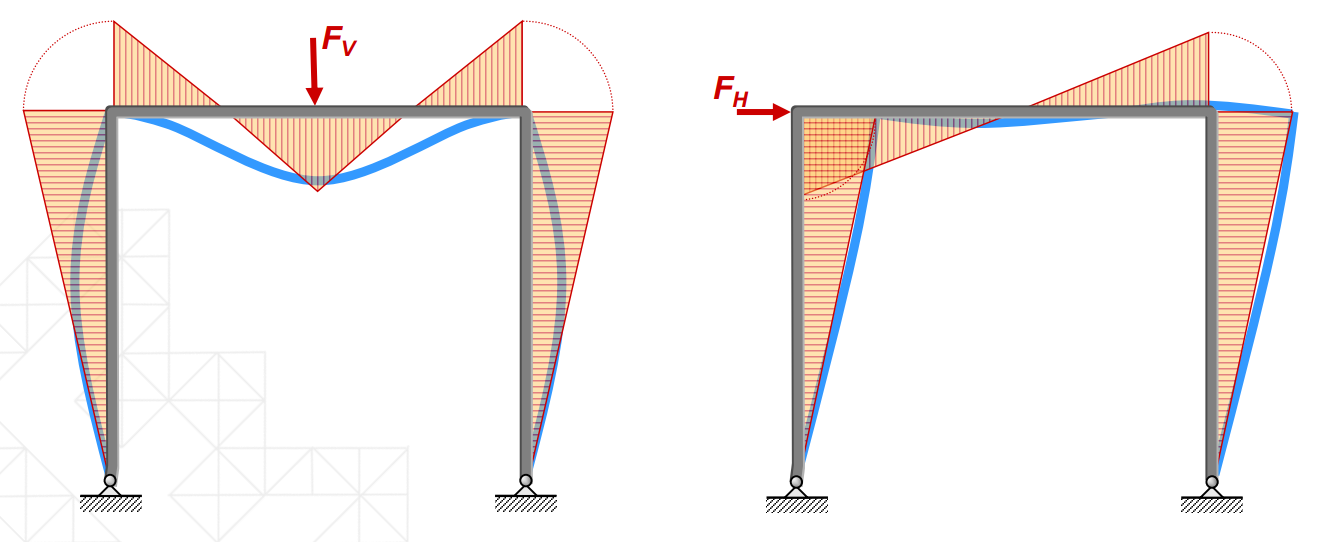
\includegraphics[width = 0.9 \textwidth]{../img/beam33.PNG}
\end{figure}
\subsubsection{Vertical Loads}
\begin{itemize}
  \item The mid span off the horizontal beam deforms downwards
  \item The corners are rigid joints
  \item The corner points are rotated (from the vertical column's POV)
  \begin{itemize}
    \item Right Corner - CCW
    \item Left Corner - CW
  \end{itemize}
  \item The bending moment is highest at the mid-span
  \item The magnitude of the bending moments at the corner (left \& right) are the same
  \begin{itemize}
    \item The arc indicates that they are the same
  \end{itemize}
\end{itemize}
\subsubsection{Horizontal Loads}
\begin{itemize}
  \item The frame is displaced to the side
  \item The corners are rigid joints
  \item Due to the rigidity of the beam, the top corners are rotated
  \item The magnitude of the bending moments at the corner (right) are the same
\end{itemize}
\subsection{Bending Moment Distribution}
By adding the contributions together, we obtain the bending moment distribution below:
\begin{figure}[H]
  \centering
  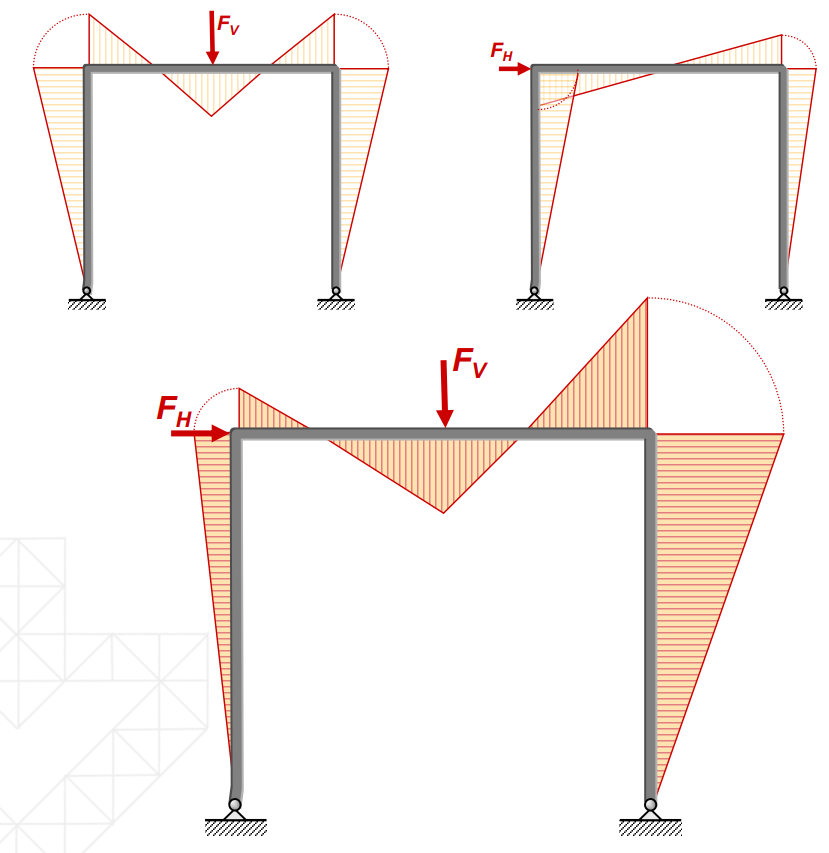
\includegraphics[width = 0.65 \textwidth]{../img/beam34.PNG}
\end{figure}
Of course, the exact distribution will depend on the relative magnitude of the two acting forces, and may vary significantly:
\begin{figure}[H]
  \centering
  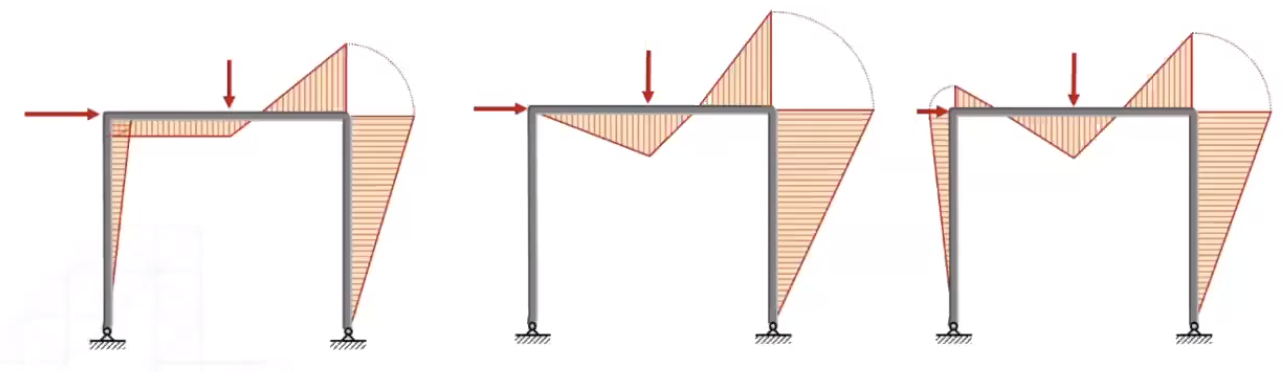
\includegraphics[width = 0.9 \textwidth]{../img/beam35.PNG}
\end{figure}
However, for any distribution, the points of maximum bending moment are located at the joints or/and at the points of application of the load.
\subsection{Plastic Hinge Sections}
In a framework with rigid joints, the points of local maximum bending moment will occur at the joints as well as under any applied loads. 
\begin{figure}[H]
  \centering
  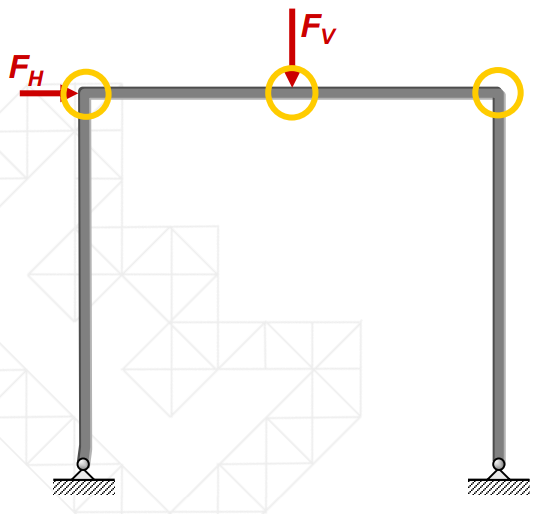
\includegraphics[width = 0.4 \textwidth]{../img/beam36.PNG}
\end{figure}
As a consequence, if plastic collapse is reached, the plastic hinges develop in some of these sections
\subsection{Possible Plastic Collapse Mechanisms}
\subsubsection{Beam Collapse:}
\begin{figure}[H]
  \centering
  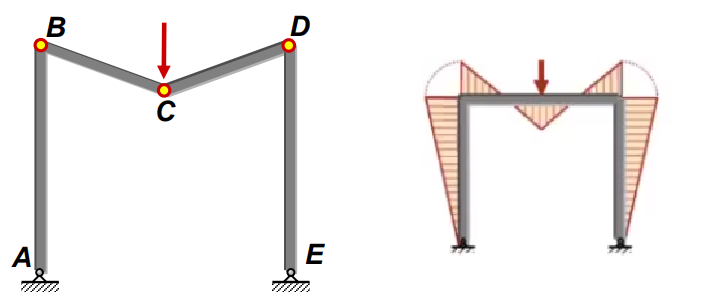
\includegraphics[width = 0.65 \textwidth]{../img/beam37.PNG}
\end{figure}
Similar mechanism to fixed-ended beams – hinges form at sections B, C and D. (vertical load much larger than horizontal)
\subsubsection{Sway Collapse:}
\begin{figure}[H]
  \centering
  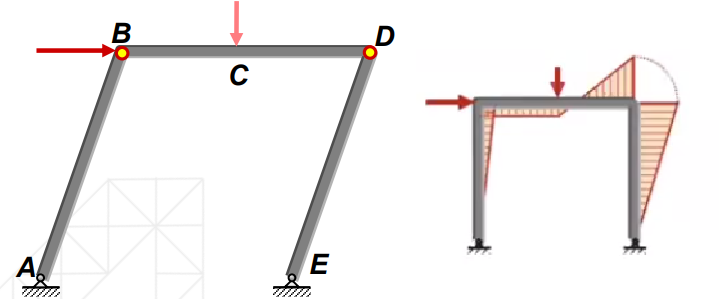
\includegraphics[width = 0.7 \textwidth]{../img/beam38.PNG}
\end{figure}
Occurs by overall sway of the frame – hinges form at sections B and D. (horizontal load much larger than vertical)
\subsubsection{Combined Beam and Sway Collapse:}
\begin{figure}[H]
  \centering
  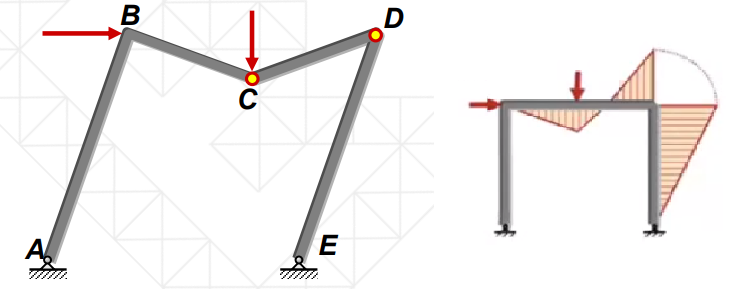
\includegraphics[width = 0.7 \textwidth]{../img/beam39.PNG}
\end{figure}
Combined beam and sway collapse – hinges form at sections C and D and section B keeps elastic. (horizontal and vertical loads comparable)
\section{Principle of Virtual Works}
\subsection{Energy}
Energy of a system is the ability of the system to do work. Energy may exist in many forms, and can be transformed from one for to another. All forms of energy can be put into two main categories: 
\begin{enumerate}
  \item Kinetic Energy - Motion (of waves, electrons, atoms, molecules, substances and objects)
  \item Potential Energy - Stored energy and energy of position (gravitational)
\end{enumerate}
\subsection{Principle of Virtual Works}
If the possible collapse mechanisms are easy to recognise (as in this case), the \textbf{principle of virtual works} can be very useful to analyse the collapse mechanisms. \\\\
Consider a structure subjected to a set of external mechanical actions. Assume for the structure a set of virtual (imaginary) displacements. The principle of virtual works states that: \\\\
\textbf{The virtual work done by the real external actions as effect of the virtual displacements is equal to the virtual work done by the real internal reactions as effect of the virtual deformations.}
\subsection{Applications to Portal Frames}
In the case of portal frames:
\begin{itemize}
  \item The set of external mechanical actions corresponds to the real forces applied to the structure;
  \item The set of internal reactions are the internal forces and moments reacting to the forces.
  \begin{itemize}
    \item Shear force
    \item Bending moment
  \end{itemize}
  \item It is convenient to chose the possible collapse mechanisms as set virtual displacements (only one of them will occur as effect of the applied load).
  \item In this case the deformations are concentrated at plastic hinges, and are the rotations produced by the internal plastic moments. 
\end{itemize}
\begin{figure}[H]
  \centering
  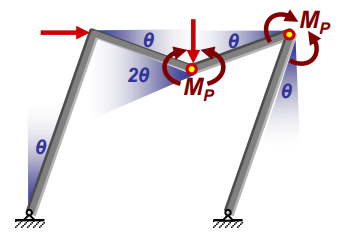
\includegraphics[width = 0.5 \textwidth]{../img/beam40.PNG}
\end{figure}
Then, the virtual work principle can be written as:
\begin{gather}
  \sum_{i=1}^{n}F_i\cdot u_i = \sum_{j=1}^{m} M_{Pj}\cdot\theta_j
\end{gather}
Where:
\begin{itemize}
  \item $F_i$ are the applied forces
  \item $M_{Pj}$ are the plastic moments at the hinges
  \item $u_i$ is the relative linear displacement
  \item $\theta_i$ is the relative angular displacement
\end{itemize}
\begin{figure}[H]
  \centering
  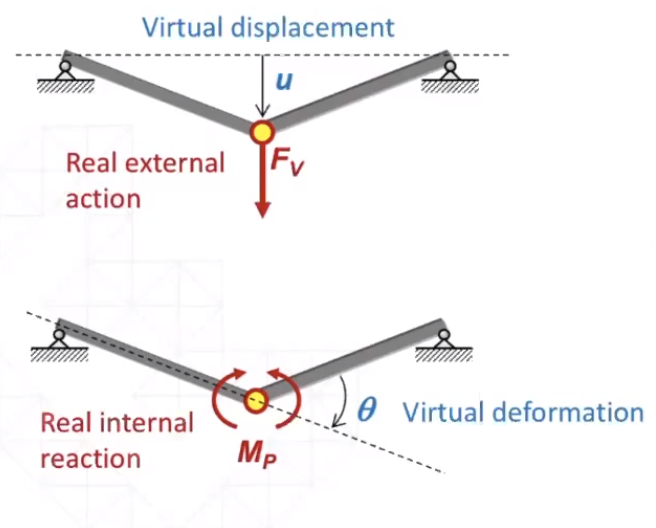
\includegraphics[width = 0.6 \textwidth]{../img/beam41.PNG}
\end{figure}
We do this to find out the level of $F_V$ such that the frame is collapse:
\begin{gather}
  F_V = f(M_P)
\end{gather}
\subsubsection{Beam Collapse:}
\begin{figure}[H]
  \centering
  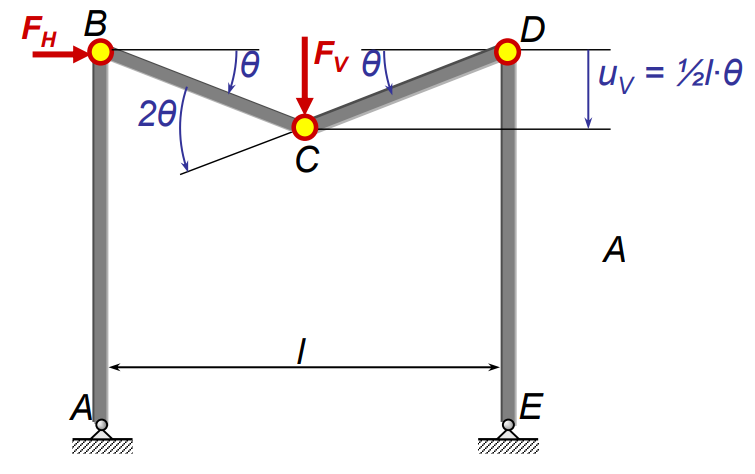
\includegraphics[width = 0.65 \textwidth]{../img/beam42.PNG}
\end{figure}
\begin{itemize}
  \item $F_H$ is ignored in this example as it is not causing any sort of displacement
  \item $F_i$ is the $F_V$ in this example, causing a vertical displacement at the middle
  \item The linear displacement $u_i$ is considered for point C
  \item The angular displacement $\theta$ is assumed to be very small $\therefore |CD| = \frac{l}{2}$ 
\end{itemize}
\begin{gather}
  F_V\cdot\frac{l}{2}\theta = M_P\cdot\theta + M_P\cdot 2\theta + M_P \cdot\theta
\end{gather}
The RHS is considered for points B,C,D respectively.
\begin{gather}
  F_V\cdot\frac{l}{2}\theta = 4M_P\cdot\theta \\
  F_V = 8\frac{M_P}{l}
\end{gather}
\subsubsection{Sway Collapse:}
\begin{figure}[H]
  \centering
  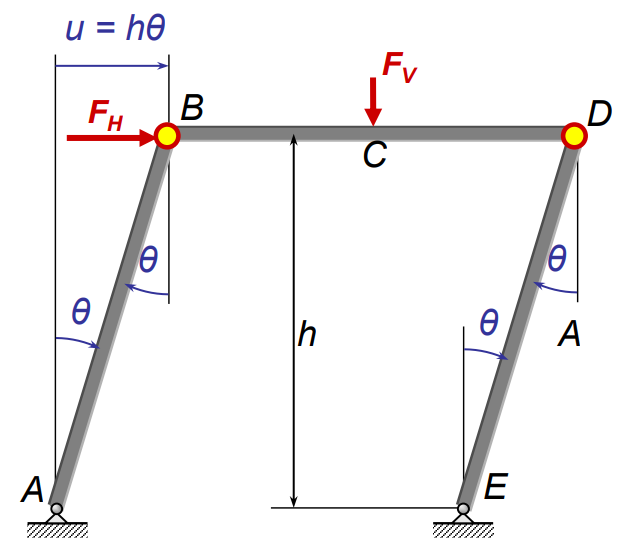
\includegraphics[width = 0.55 \textwidth]{../img/beam43.PNG}
\end{figure}
\begin{itemize}
  \item $F_V$ is ignored in this example as it is not causing any sort of displacement
  \item $F_i = F_H$, causing a horizontal displacement
  \item $u_i = h\theta$
  \item $\theta \approxeq 0 \therefore |CD| = \frac{l}{2}$ 
\end{itemize}
\begin{gather}
  F_H\cdot h\theta = M_P\cdot\theta + M_P\cdot\theta 
\end{gather}
The RHS is considered for points B and D.
\begin{gather}
  F_H\cdot h\theta = 2M_P\cdot\theta \\
  F_H = 2\frac{M_P}{h}
\end{gather}
\subsubsection{Combined Collapse:}
\begin{figure}[H]
  \centering
  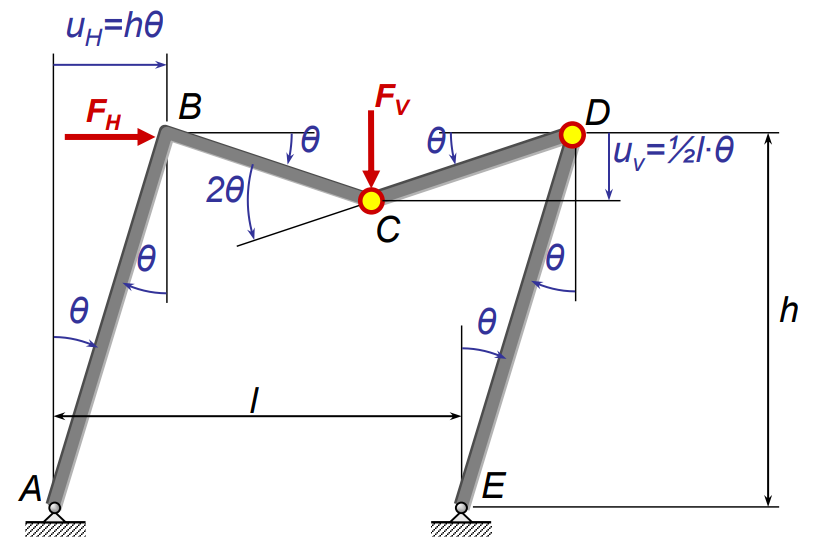
\includegraphics[width = 0.6 \textwidth]{../img/beam44.PNG}
\end{figure}
\begin{itemize}
  \item Only points C and D are under collapse
  \item $F_i = F_H \ \text{and} \ F_V$
  \item $u_h = h\theta$
  \item $u_v = \frac{l}{2}\theta$
  \item $\theta \approxeq 0 \therefore |CD| = \frac{l}{2}$ 
\end{itemize}
\begin{gather}
  F_Hh + F_V\frac{l}{2} = 4M_P
\end{gather}
\subsection{Collapse Mechanism}
The collapse mechanism of the portal frame, under the effect of the external forces considered is \textbf{the one that requires lower critical forces} (the one that is reached first).
\section{Portal Frames with Fixed Bases}
Consider a flat-roofed portal frame with pinned feet, carrying a vertical concentrated load $F_V$ at the centre of the beam and an horizontal concentrated load $F_H$ at the top of one column.
\begin{figure}[H]
  \centering
  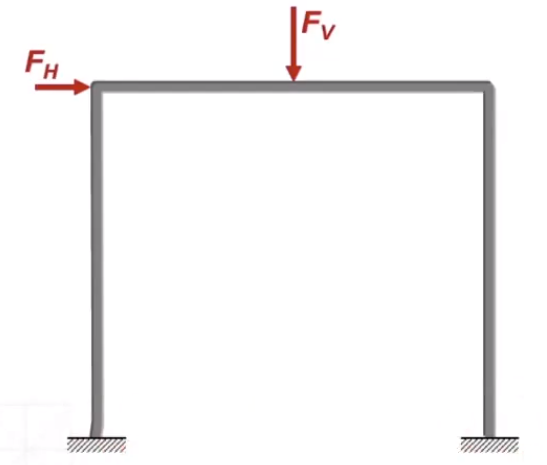
\includegraphics[width = 0.4 \textwidth]{../img/beam45.PNG}
\end{figure}
\subsection{Deformations and Bending Moments}
In this case, the deformations and bending moment distribution produced by the horizontal and vertical loads considered independently are respectively:
\begin{figure}[H]
  \centering
  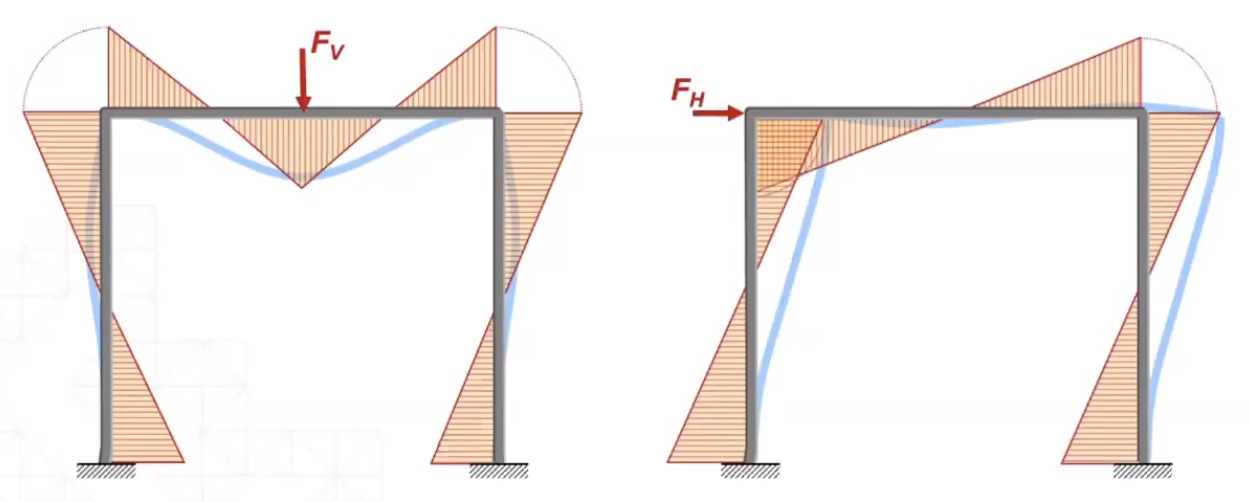
\includegraphics[width = 0.9 \textwidth]{../img/beam46.PNG}
\end{figure}
\subsection{Bending Moment Distribution}
By adding the contributions together, we obtain the bending moment distribution below:
\begin{figure}[H]
  \centering
  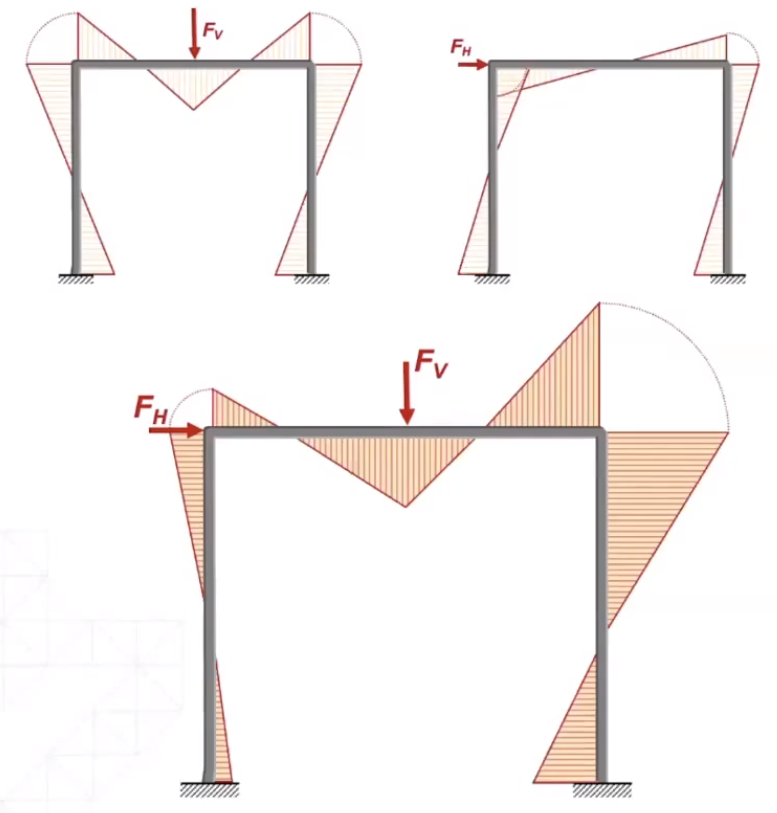
\includegraphics[width = 0.65 \textwidth]{../img/beam47.PNG}
\end{figure}
Again, the exact distribution will depend on the relative magnitude of the two acting forces, and may vary significantly (with one column left unstressed in one of the possible configurations):
\begin{figure}[H]
  \centering
  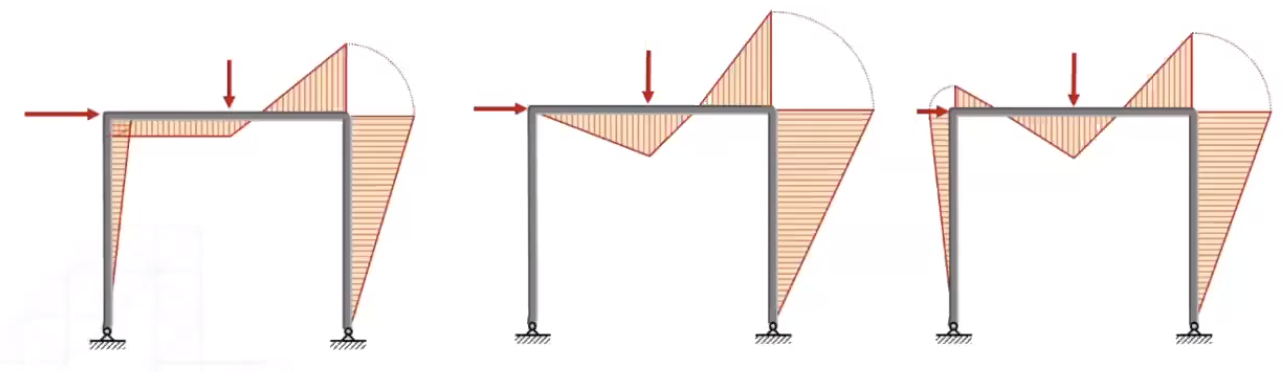
\includegraphics[width = 0.9 \textwidth]{../img/beam35.PNG}
\end{figure}
It is confirmed again that the sections of maximum bending moment are located at the joints or/and at the points of application of the load. Therefore, the plastic hinges develop in some of these sections.
\subsection{Possible Plastic Collapse Mechanisms}
\subsubsection{Beam Collapse:}
\begin{figure}[H]
  \centering
  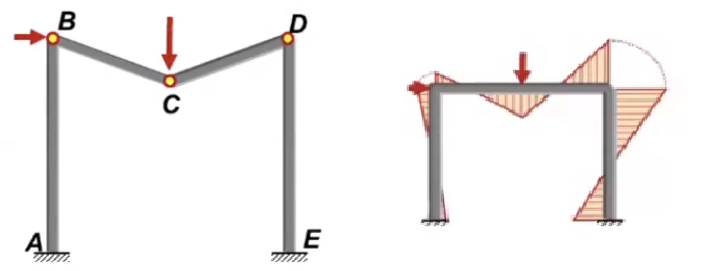
\includegraphics[width = 0.65 \textwidth]{../img/beam49.PNG}
\end{figure}
Similar mechanism to fixed-ended beams – hinges form at sections B, C and D. (occurs when vertical load is dominant)
\subsubsection{Sway Collapse:}
\begin{figure}[H]
  \centering
  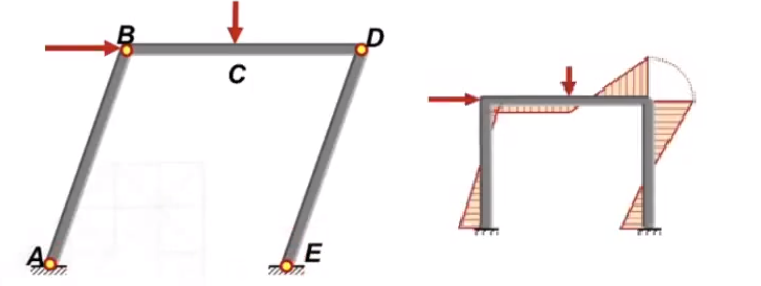
\includegraphics[width = 0.7 \textwidth]{../img/beam50.PNG}
\end{figure}
Occurs by overall sway of the frame – hinges form at sections A, B, D and E. (due to a dominant horizontal load)
\subsubsection{Combined Beam and Sway Collapse:}
\begin{figure}[H]
  \centering
  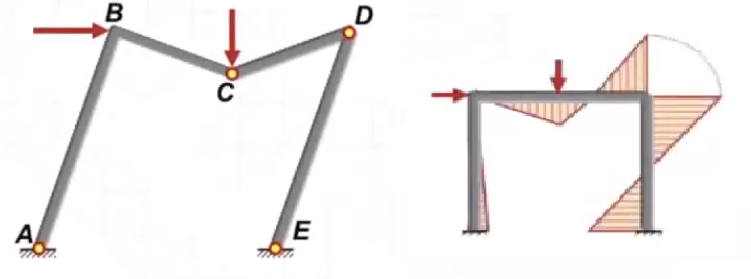
\includegraphics[width = 0.7 \textwidth]{../img/beam51.PNG}
\end{figure}
Combined beam and sway collapse – hinges form at sections A, C, D and E and section B keeps elastic. (horizontal and vertical loads comparable)
\subsubsection{Beam Collapse:}
\begin{figure}[H]
  \centering
  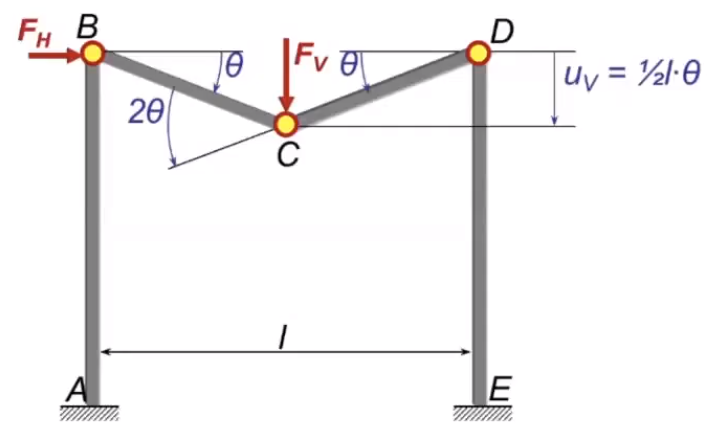
\includegraphics[width = 0.6 \textwidth]{../img/beam52.PNG}
\end{figure}
\begin{gather}
  F_V = 8\frac{M_P}{l}
\end{gather}
\subsubsection{Sway Collapse:}
\begin{figure}[H]
  \centering
  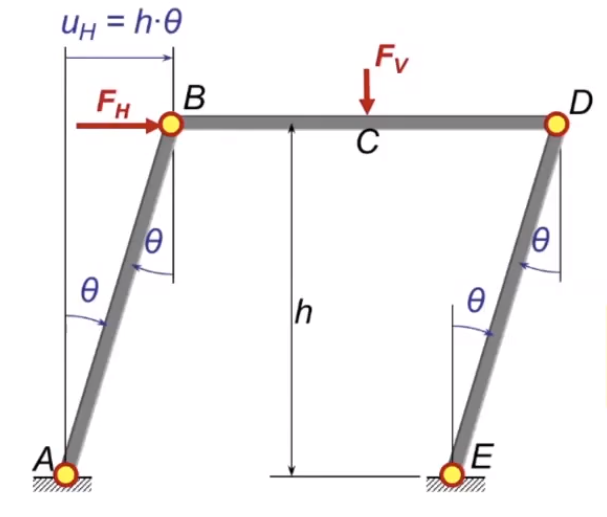
\includegraphics[width = 0.5 \textwidth]{../img/beam53.PNG}
\end{figure}
\begin{gather}
  F_H \cdot h\theta = M_P\theta + M_P\theta + M_P\theta + M_P\theta \\
  F_H \cdot h\theta 4M_P\theta \\
  F_H = 4\frac{M_P}{h}
\end{gather}
\subsubsection{Combined Collapse:}
\begin{figure}[H]
  \centering
  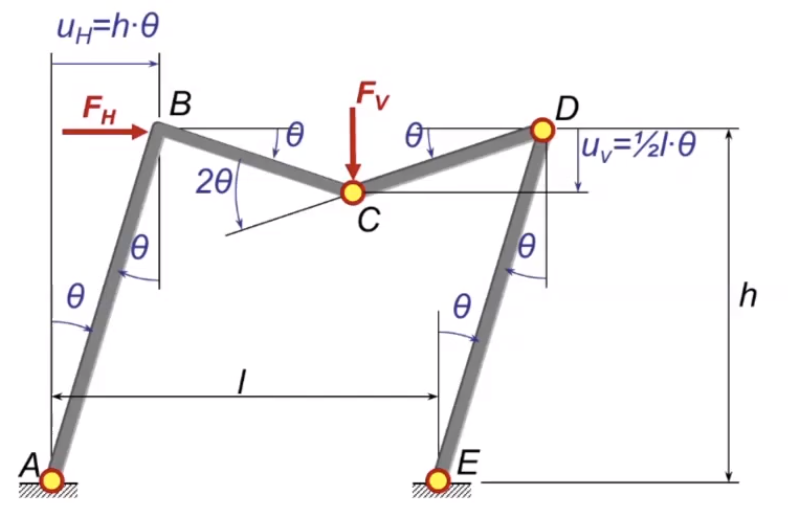
\includegraphics[width = 0.65 \textwidth]{../img/beam54.PNG}
\end{figure}
\begin{gather}
  F_Hh + F_V\frac{l}{2} = 6M_P
\end{gather}
\subsection*{Example}
\begin{figure}[H]
  \centering
  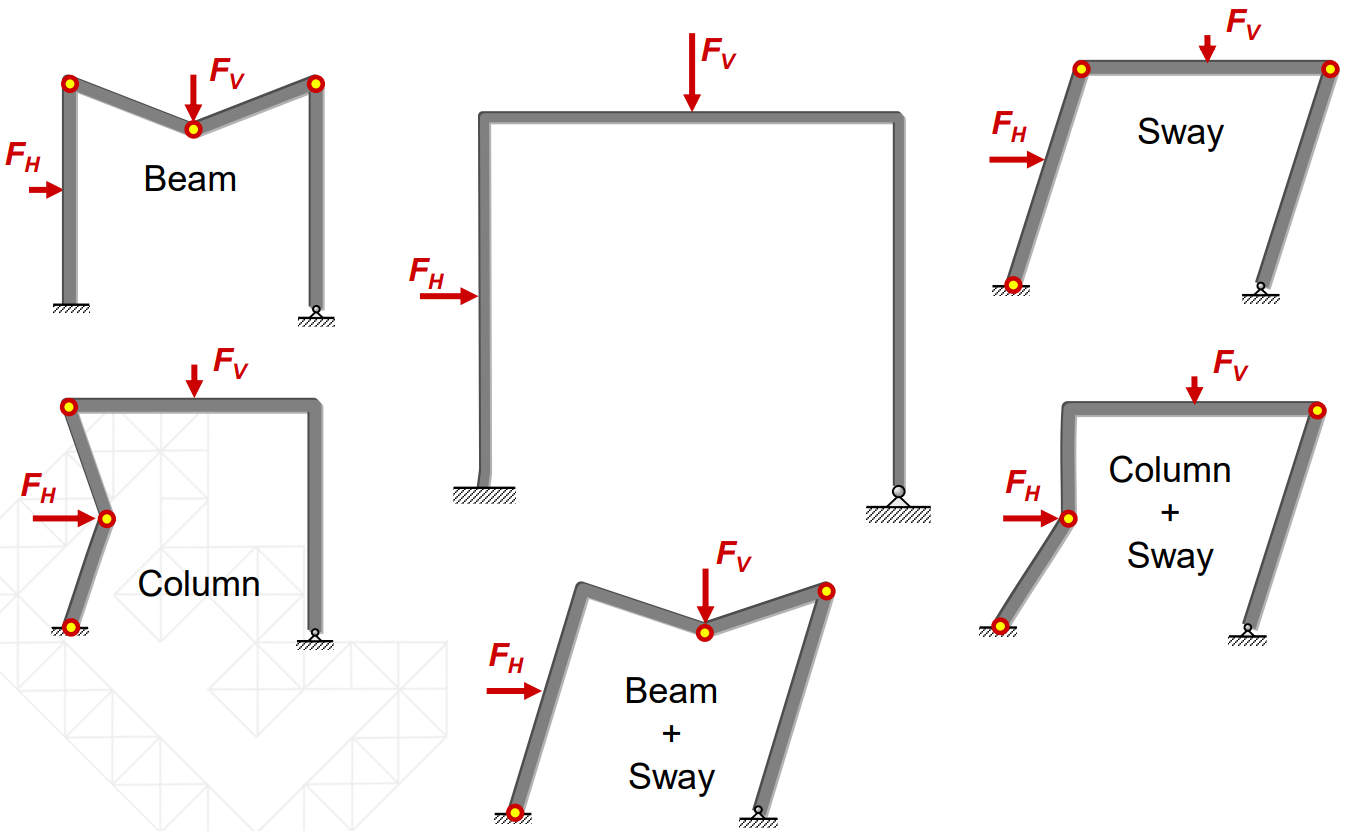
\includegraphics[width = 1 \textwidth]{../img/beam55.PNG}
\end{figure}
These are all possible modes of collapse. Find out which mode is the easiest to occur and under what level of load.
\begin{figure}[H]
  \centering
  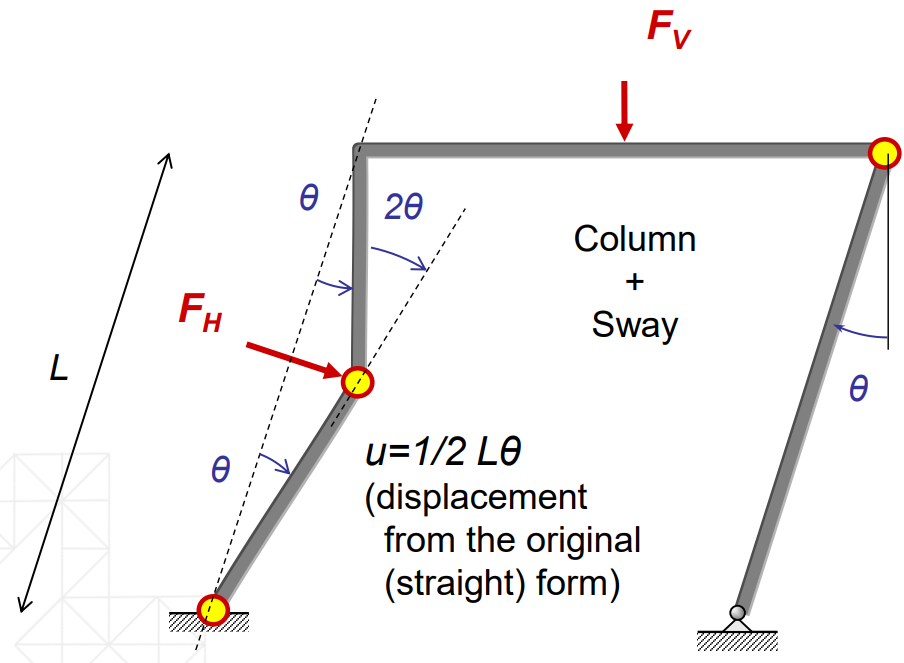
\includegraphics[width = 0.65 \textwidth]{../img/beam56.PNG}
\end{figure}
Other modes are the same as previous examples.
\end{document}